% -*- TeX -*-
%
% ----------------------------------------------------------------------
%
%                           Brad T. Aagaard
%                        U.S. Geological Survey
%
% {LicenseText}
%
% ----------------------------------------------------------------------
%
\documentclass[pdftex,cig,slideColor]{pp4slides}
\usepackage{amsmath}
\usepackage{array}
\usepackage{xspace}
\usepackage{multirow}
\usepackage{ulem}

\newcommand{\newfeature}[1]{{\color{blue}#1}}

\renewcommand{\movielink}[2]{\href{run:#1.avi}{#2}}

\title{PyLith 1.5 Tutorial}
\subtitle{}
\author{Brad Aagaard\\[10pt]
  Charles Williams, Matthew Knepley,\\
  and Surendra Somala}
\institution{\includegraphics[height=2cm]{../../logos/cig}}
\date{June 14, 2010}

% --------------------------------------------------------- DOCUMENT
\begin{document}

% ------------------------------------------------------------ SLIDE
\maketitle

% ------------------------------------------------------------ SLIDE
\foilhead{Crustal Deformation Modeling}
  \summary{Overview of workflow for typical research problem}

  \vfill
  \begin{center}
    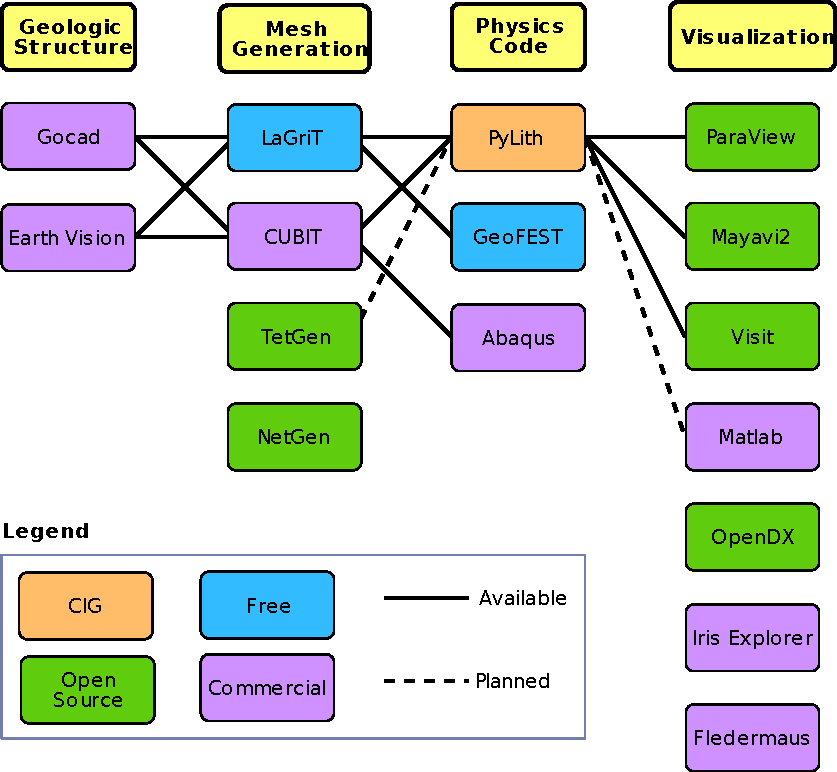
\includegraphics[scale=1.15]{figs/workflow}
  \end{center}
  \vfill

\bgadd{\vspace*{7.9in}%
  \begin{center}%
    \includegraphics[height=14mm]{../../logos/cig}
  \end{center}}

% ------------------------------------------------------------ SLIDE
\foilhead{Ingredients for Running PyLith}

  \begin{itemize}
  \item Simulation parameters
  \item Finite-element mesh
    \begin{itemize}
    \item Mesh exported from LaGriT
    \item Mesh exported from CUBIT
    \item Mesh constructed by hand (PyLith mesh ASCII format)
    \end{itemize}
  \item Spatial databases for physical properties, boundary
    conditions, and rupture parameters
    \begin{itemize}
    \item SCEC CVM-H or USGS Bay Area Velocity model
    \item Simple ASCII files
    \end{itemize}
  \end{itemize}

% ------------------------------------------------------------ SLIDE
\foilhead{Spatial Databases}
  \summary{User-specified field/value in space}

  \begin{itemize}
 \item Examples
    \begin{itemize}
    \item Uniform value for Dirichlet (0-D)
    \item Piecewise linear variation in tractions for Neumann BC (1-D)
    \item SCEC CVM-H seismic velocity model (3-D)
    \end{itemize}
  \item Generally independent of discretization for problem
  \item Available spatial databases
    \begin{description}
    \item[UniformDB] Optimized for uniform value
    \item[SimpleDB] Simple ASCII files (0-D, 1-D, 2-D, or 3-D)
    \item[SCECCVMH] SCEC CVM-H seismic velocity model v5.3
    \item[ZeroDispDB] Special case of UniformDB
    \end{description}
 \end{itemize}


  % ------------------------------------------------------------ SLIDE
\foilhead{Features in PyLith 1.5}
  \summary{Enhancements and new features in \newfeature{blue}}

  \begin{itemize}
  \item Time integration schemes and elasticity formulations
    \begin{itemize}
    \item Implicit for quasi-static problems (neglect inertial terms)
      \begin{itemize}
      \item Infinitesimal strains
      \item \newfeature{Small strains}
      \end{itemize}
    \item Explicit for dynamic problems
      \begin{itemize}
      \item Infinitesimal strains with sparse system Jacobian
      \item \newfeature{Infinitesimal strains with lumped system Jacobian}
      \item \newfeature{Small strains with sparse system Jacobian}
      \end{itemize}
    \end{itemize}
  \item Bulk constitutive models
    \begin{itemize}
    \item Elastic model (1-D, 2-D, and 3-D)
    \item Linear and Generalized Maxwell viscoelastic models (3-D)
    \item Power-law viscoelastic model (3-D)
    \item \newfeature{Linear Maxwell viscoelastic model (2-D)}
    \item \newfeature{Drucker-Prager elastoplastic model (3-D)}
    \end{itemize}
 \end{itemize}


% ------------------------------------------------------------ SLIDE
\foilhead{Features in PyLith 1.5 (cont.)}
  \summary{Enhancements and new features in \newfeature{blue}}

  \begin{itemize}
  \item Boundary and interface conditions
    \begin{itemize}
    \item Time-dependent Dirichlet boundary conditions
    \item Time-dependent Neumann (traction) boundary conditions
    \item Absorbing boundary conditions
    \item Kinematic (prescribed slip) fault interfaces w/multiple ruptures
    \item \newfeature{Dynamic (friction) fault interfaces}
    \item Time-dependent point forces
    \item Gravitational body forces
    \end{itemize}
  \item Fault constitutive models
    \begin{itemize}
    \item \newfeature{Static friction}
    \item \newfeature{Linear slip-weakening}
    \item \newfeature{Dieterich-Ruina rate and state friction w/ageing
      law}
   \end{itemize}
 \end{itemize}


% ------------------------------------------------------------ SLIDE
\foilhead{Features in PyLith 1.5 (cont.)}
  \summary{Enhancements and new features in \newfeature{blue}}

  \begin{itemize}
  \item Automatic and user-controlled time stepping
  \item Ability to specify initial stress state
  \item Importing meshes
    \begin{itemize}
    \item LaGriT: GMV/Pset
    \item CUBIT: Exodus II
    \item ASCII: PyLith mesh ASCII format (intended for toy problems only)
    \end{itemize}
  \item Output: VTK files
    \begin{itemize}
    \item Solution over volume
    \item Solution over surface boundary
    \item State variables (e.g., stress and strain) for each material
    \item Fault information (e.g., slip and tractions)
    \end{itemize}
  \item Automatic conversion of units for all parameters
  \end{itemize}
  
% ------------------------------------------------------------ SLIDE
\foilhead{PyLith 1.5: Under-the-hood Improvements}
  \summary{}

  \begin{itemize}
  \item Additional cleanup of C++ code
  \item Optimization of several modules
    \begin{itemize}
    \item Mesh distribution among processors
    \item Integration of elasticity terms
    \end{itemize}
  \item Ability to use algebraic multigrid preconditioners
 \end{itemize}
    

% ------------------------------------------------------------ SLIDE
\foilhead{Time-Dependent Boundary Conditions}
  \summary{Dirichlet, Neumann, and Point Forces}
  
  \begin{equation*}
    \begin{split}
      f(\vec{x}) =& \\[10pt]
      & \begin{array}{lr}
        f_{0}(\vec{x}) + & \textrm{{\tt db\_initial}}\\[10pt]
        \dot{f}_{1}(\vec{x}) (t-t_{1}(\vec{x})) + & \textrm{{\tt db\_rate}}\\[10pt]
        f_{2}(\vec{x})a(t-t_{2}(\vec{x})) & \textrm{{\tt db\_change}}
      \end{array}
    \end{split}
  \end{equation*}
  \vfill
  \begin{description}
  \item[db\_initial] Initial value (constant in time)
  \item[db\_rate] Constant rate of change (spatially variable start time)
  \item[db\_change] Time history (spatially variable amplitude and
    start time)
  \end{description}

 
% ------------------------------------------------------------ SLIDE
\foilhead{PyLith as a Hierarchy of Components}
  \summary{Components are the basic building blocks}

  \vfill
  \begin{center}
    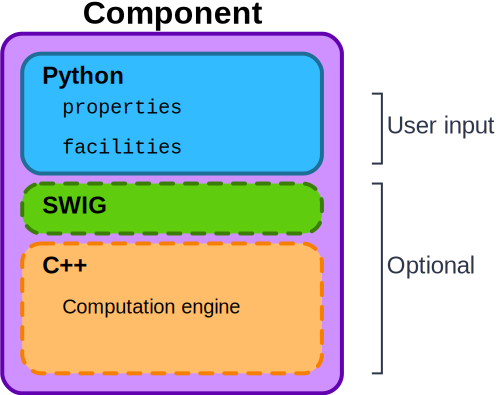
\includegraphics[scale=1.0]{figs/component}
  \end{center}  
  \vfill

% ------------------------------------------------------------ SLIDE
\foilhead{PyLith as a Hierarchy of Components}
  \summary{PyLith Application and Time-Dependent Problem}

  \vfill
  \begin{center}
    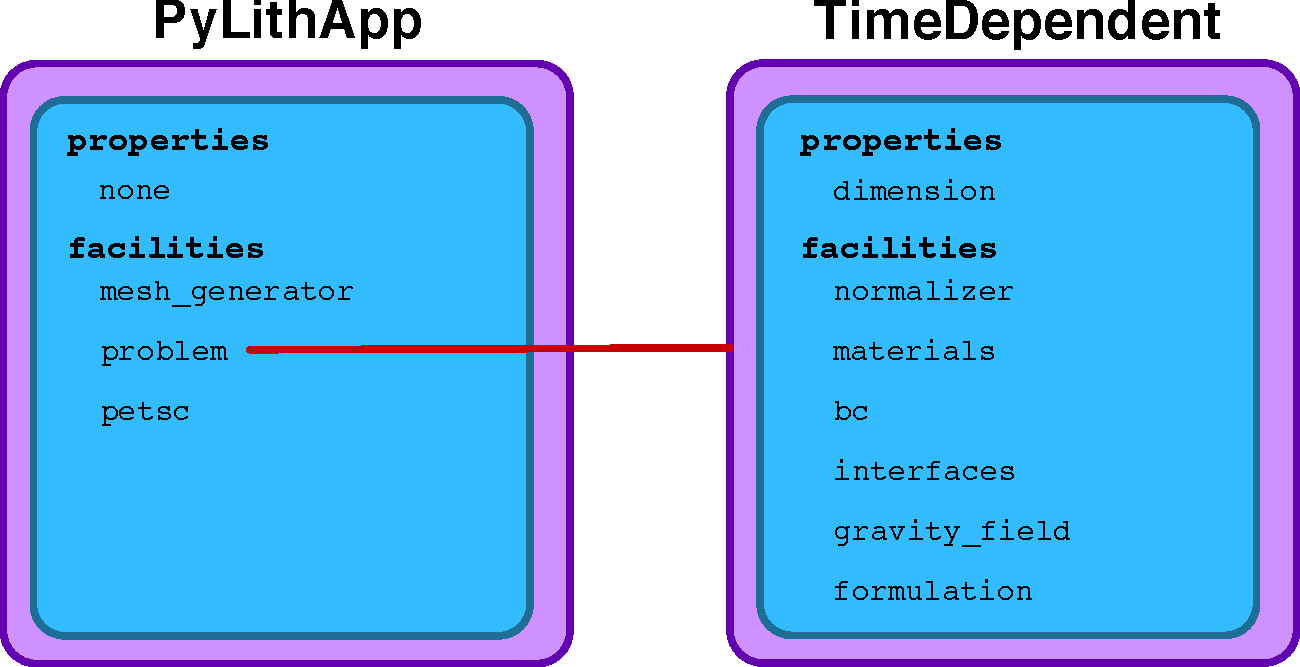
\includegraphics[scale=1.0]{figs/pylithapp}
  \end{center}  
  \vfill

% ------------------------------------------------------------ SLIDE
\foilhead{PyLith as a Hierarchy of Components}
  \summary{Fault with kinematic (prescribed slip) earthquake rupture}

  \vfill
  \begin{center}
    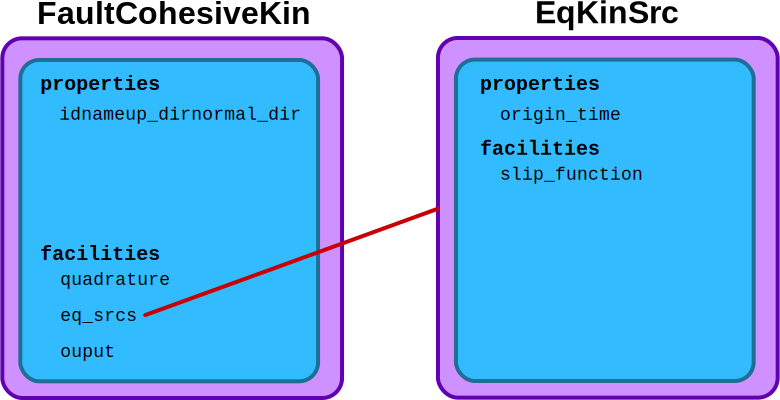
\includegraphics[scale=1.0]{figs/faultcohesivekin}
  \end{center}  
  \vfill

% ------------------------------------------------------------ SLIDE
\foilhead{PyLith Application Flow}
  \summary{}
 {\small
  \begin{minipage}[t]{3.75in}
    {\bf PyLithApp}\\[8pt]
    \begin{verbatim}
  main()
    mesher.create()
    problem.initialize()
    problem.run()
    \end{verbatim}
    \vspace*{20pt}
    {\bf TimeDependent (Problem)}\\[8pt]
    \begin{verbatim}
  initialize()
    formulation.initialize()

  run()
    while (t < totalTime)
      dt = formulation.getTimeStep()
      formulation.prestep()
      formulation.step()
      formulation.poststep()
\end{verbatim}
  \end{minipage}
  \hfill
  \begin{minipage}[t]{3.75in}
    {\bf Implicit (Formulation)}\\[8pt]
    \begin{verbatim}
  initialize()

  prestep()
    set constraints

  step()
    calculate residual
    solve for displacement increment

  poststep()
    update displacement field
    write output
\end{verbatim}
  \end{minipage}
}

% ------------------------------------------------------------ SLIDE
\foilhead{Ingredients for Running PyLith}

  \begin{itemize}
  \item Simulation parameters
    \begin{itemize}
    \item {\tt .cfg} ASCII files
    \item {\tt pylithapp.cfg} always read if it exists
    \item Command line arguments
    \end{itemize}
  \item Finite-element mesh
    \begin{itemize}
    \item Mesh exported from LaGriT
    \item Mesh exported from CUBIT
    \item Mesh constructed by hand (PyLith mesh ASCII format)
    \end{itemize}
  \item Spatial databases for physical properties, boundary
    conditions, and rupture parameters
  \end{itemize}

% ------------------------------------------------------------ SLIDE
\foilhead{Example: {\tt 3d/hex8 step01.cfg}}
  \summary{Compression and shear via prescribed displacements}

  \vfill
  \begin{center}
    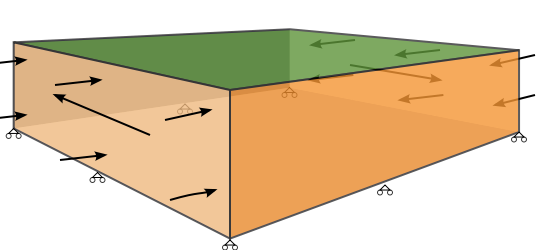
\includegraphics[scale=1.0]{figs/step01_diagram}
  \end{center}
  \vfill

% ------------------------------------------------------------ SLIDE
\foilhead{\ }

\vspace*{-1.0in}%
{\large Example: {\tt 3d/hex8 step01.cfg}}\\
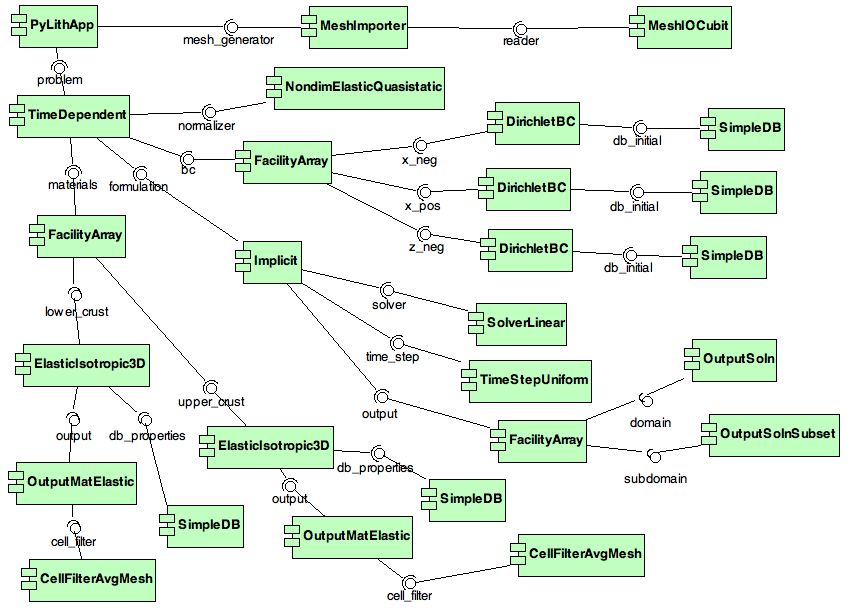
\includegraphics[scale=0.84]{figs/step01_components}

% ------------------------------------------------------------ SLIDE
\foilhead{Example: {\tt 3d/hex8 step01.cfg}}
  \summary{}

  \begin{minipage}[t]{4in}
    {\centering {\bf Input}}
    \begin{itemize}
    \item Simulation parameters
      \begin{itemize}
      \item {\tt pylithapp.cfg}
      \item {\tt step01.cfg}
      \end{itemize}
    \item CUBIT Mesh: \\ {\tt mesh\_hex8\_1000m.mesh}
    \item Spatial databases
      \begin{itemize}
      \item {\tt mat\_elastic.spatialdb}
      \item {\tt axialdisp.spatialdb}
      \end{itemize}
    \end{itemize}
  \end{minipage}
  \hfill
  \begin{minipage}[t]{4.75in}
    {\centering {\bf Output}}
    \begin{itemize}
   \item Displacement field
      \begin{itemize}
      \item {\tt step01\_t000000.vtk}
      \item {\tt step01-groundsurf\_t000000.vtk}
      \end{itemize}
    \item State variables
      \begin{itemize}
      \item Upper crust (elastic)
        \begin{itemize}
        \item {\tt step01-statevars\_info.vtk} (physical properties)
        \item {\tt step01-statevars\_t000000.vtk} (stress and strain)
        \end{itemize}
      \item Lower crust (elastic)
        \begin{itemize}
        \item {\tt step01-statevars\_info.vtk} (physical properties)
        \item {\tt step01-statevars\_t000000.vtk} (stress and strain)
        \end{itemize}
      \end{itemize}
    \end{itemize}
  \end{minipage}   

% ------------------------------------------------------------ SLIDE
\foilhead{Example: {\tt 3d/hex8 step06.cfg}}
  \summary{Creep and repeated rupture on a strike-slip fault}

  \vfill
  \begin{center}
    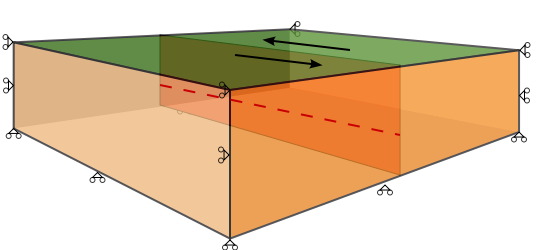
\includegraphics[scale=1.0]{figs/step06_diagram}
  \end{center}
  \vfill

% ------------------------------------------------------------ SLIDE
\foilhead{Example: {\tt 3d/hex8 step06.cfg}}
  \summary{Creep and repeated rupture on a strike-slip fault}
 
\movie{0.5in}{0.0in}{8.0in}{5.7778in}{movies/step06}%


% ------------------------------------------------------------ SLIDE
\foilhead{Example: {\tt 3d/hex8 savageprescott.cfg}}
 \summary{}

{\small
 \hspace*{-0.5in}
  \begin{minipage}[t]{4.5in}
    {\centering {\bf Input}}
    \begin{itemize}
    \item Simulation parameters
      \begin{itemize}
      \item {\tt pylithapp.cfg}
      \item {\tt step06.cfg}
      \end{itemize}
    \item Mesh: {\tt mesh\_hex8\_1000m.exo}
    \item Spatial databases
      \begin{itemize}
      \item {\tt mat\_elastic.spatialdb}
      \item {\tt mat\_maxwell.spatialdb}
      \item {\tt finalslip\_rupture.spatialdb}
      \item {\tt sliptime.spatialdb}
      \item {\tt sliprate\_creep.spatialdb}
      \end{itemize}
    \end{itemize}
  \end{minipage}
  \hfill
  \begin{minipage}[t]{4.75in}
    {\centering {\bf Output}}
    \begin{itemize}
   \item Displacement field
      \begin{itemize}
      \item {\tt step06\_tNNNN.vtk}
      \item {\tt step06-groundsurf\_tNNNN.vtk}
      \end{itemize}
    \item State variables
      \begin{itemize}
      \item Upper crust (elastic)
        \begin{itemize}
        \item {\tt step06-upper\_crust\_info.vtk}
        \item {\tt step06-upper\_crust\_tNNNN.vtk}
        \end{itemize}
      \item Lower crust (viscoelastic)
        \begin{itemize}
        \item {\tt step06-lower\_crust\_info.vtk}
        \item {\tt step06-lower\_crust\_tNNNN.vtk}
        \end{itemize}
      \end{itemize}
    \item Fault
      \begin{itemize}
      \item {\tt step06-fault\_info.vtk}
      \item {\tt step06-fault\_tNNNN.vtk}
      \end{itemize}
    \end{itemize}
  \end{minipage}   
}

% ------------------------------------------------------------ SLIDE
\foilhead{Useful Tips/Tricks}
  \summary{}

  \begin{itemize}
  \item {\tt pylithinfo [--verbose] [PyLith args]}\\
    Dumps all parameters with their current values to text file
  \item Command line arguments
    \begin{itemize}
    \item {\tt --help}
    \item {\tt --help-components}
    \item {\tt --help-properties}
    \item {\tt --petsc.start\_in\_debugger} (run in xterm)
    \item {\tt --nodes=N} (to run on N processors on local machine)
    \end{itemize}
  \item PyLith User Manual
  \item CIG Short-Term Tectonics mailing list\\
    {\tt cig-short@geodynamics.org}
  \item CIG bug tracking system\\
    {\tt http://www.geodynamics.org/roundup}
  \end{itemize}


% ======================================================================
\end{document}


% End of file
